% --
% theory

\section{Theory}\label{sec:nn_theory}
\thesisStateNotReady
The theory provided in this sections merely focuses on the used neural network architectures and some basic theory elements in neural networks.
The most basic element in neural networks is described here as node, an abstract element, usually illustrated as circle, that defines input and output connections from and to other nodes within the network.
The connections from and to a node are multiplications with scalar values, denoted as weight.
Each node usually incorporates an additive term, denoted as bias term.
All weights and bias terms are forming the parameters of a network and can be trained through back-propagation.
The output of a node is a scalar computed from all inputs and mapped with a non-linear function denoted as activation function.
A neural network can consist of thousand of nodes in each possible constellation of connections.
In this thesis, the focus is only on single directional connections (no bidirectional connections).
The structure of a neural network is defined by its layers, where a layer is a set of nodes with specific connection properties that receive inputs from the previous layer and output connections to the next layer.
For example, a neural network consists one convolutional layer followed by three fully connected layers.
The last layer of a neural network represents for instance the class labels of a classification tasks.
A loss function computes the difference between the predicted and the actual class label during training and is essential for the backpropagation algorithm that updates each parameter in the network through the gradients of the obtained error.


% --
% activation functions

\subsection{Activation Functions}\label{sec:nn_theory_acti}
Activation functions for neural networks of a node in a current layer are non-linear functions that usually maps the sum of the weighted inputs from nodes in a previous layer to a single output value $z$ as following:
\begin{equation}\label{eq:nn_theory_acti}
  z = h(w \, x^T)
\end{equation}
where $h$ is the activation function, $w \in \R^n$ is an weight vector and $x \in \R^n$ an input vector for one specific node.
The output of each node in a current layer is further connected to other nodes in the next layer and builds up the neural network.
The constraint of an activation function is, that an easy computable derivative of this function exist, in order to backpropagate gradients.

The most famous activation function nowadays is the RELU function:
\begin{equation}\label{eq:nn_theory_relu}
  z = \max{(0, a)}
\end{equation}
with $a \in \R$ as input to the activation function.
The big advantage is that this function and its subgradients are very easy and fast to compute.
The two other activation functions that are used in wavenets are the sigmoid function:
\begin{equation}\label{eq:nn_theory_sigmoid}
  z = \frac{1}{1 + \exp{-x}}
\end{equation}
and the tanh functions:
\begin{equation}\label{eq:nn_theory_tanh}
  z = \frac{\exp{x} - \exp{-x}}{\exp{x} + \exp{-x}}
\end{equation}


% --
% fully connected

\subsection{Fully Connected Layer}
A fully connected (FC) layer is the simplest layer type in neural networks.
Each node from the previous layer is connected in forward direction to all nodes in the FC layer and each node in the FC layer is further connected to all nodes in the next layer.
Further each connection has one trainable weight and each node has a bias term.
A simple FC layer is illustrated in \rfig{nn_theory_fc}.
% fc
\begin{figure}[!ht]
  \centering
    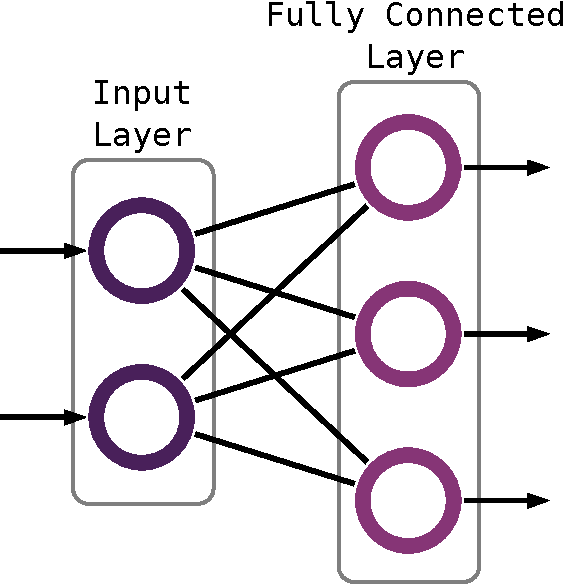
\includegraphics[width=0.30\textwidth]{./4_nn/figs/nn_theory_fc.eps}
  \caption{Basic fully connected layer with 3 nodes, receiving connections from 2 input nodes and outputing connections to 2 output nodes.}
  \label{fig:nn_theory_fc}
\end{figure}
\FloatBarrier
\noindent
In one node usually following computation is processed:
\begin{equation}
  z = h(w \, x^T + b)
\end{equation}
with the same notations as in \req{nn_theory_acti} and an additional bias term $b \in \R$.


% --
% cnn

\subsection{Convolutional Layers}\label{sec:nn_theory_cnn}
Convolutional layers are the fundament of every Covolutional Neural Networks (CNN) as already discussed in \rsec{prev_nn_cnn}.
They use convolutional filters on small areas of the input data, so that spatial information is retrieved.
Those convolutional filters are also called kernels and illustrated in case of images as rectangle in 2D space with kernel width $k_w$ and height $k_h$.
The kernel is shifted over its input map in each axis with an operation called \emph{stride}, denoted as $s$, and produce a output map through convolution.
The output dimension $o_d$ for striding along this axis with $s_d$ and kernel size for that axis $k_d$ over the input dimension $i_d$ can be computed as:
\begin{equation}\label{eq:nn_theory_cnn_}
  o_d = \floor*{\frac{i_d + p_d - k_d}{s_d} + 1}
\end{equation}
where $p_d$ is additionally a \emph{padding} term, where for instance for in zero-padding, zeros are added on both sides of the input dimension.
For example if a $16 \times 16$ image is convoluted by a $5 \times 5$ kernel with stride $1$ in each direction and no padding, the output image is $12 \times 12$.
The padding operation has usually the purpose to keep a the output and input dimension the same.
This is used for instance in residual neural networks, where the input to convolutional layers of a block, is bypassed and added to the output of this block again.
Being able to compute the addition operation from input and output of the residual block, their dimensions must be the same.
However in most convolutional network applications without residual blocks, it is preferred not to pad the image, so that dimensions are reduced hence parameters and multiplications saved.
Further there exist some special convolutional layers designed to reduce the dimensions (subsampling), such as a Max-Pooling layer. 

As already mentioned above CNNs are defined with the amount of input and output channels (feature maps), the kernel size, the stride of the kernel and some other specialties like dilation.
However it is not immediately clear from those parameter, how many convolutional filters are applied and what how the output feature maps are calculated exactly.
The amount of convolutional filters is in most practical examples always:
\begin{equation}\label{eq:nn_theory_n_filters}
  \#k = i \cdot j
\end{equation}
where $i$ and $j$ is the amount of input and output channels respectively.
Each kernel produces an output map, but the idea is to constraint the number of output maps $\#k$ to the defined output channels $j$.
This is usually done by summing up all output maps of input channels $i$ for one output channel $j$:
\begin{equation}
  o_j = \sum_{i} k_{i, j} * x_i
\end{equation}
where $o_j$ is the j-th feature map, $k_{i, j}$ the kernel of $i$ and $j$ and $x_i$ the i-th input channel.
A gaphical example of this procedure is shown in \rfig{nn_theory_cnn_basics}.
% cnn basics
\begin{figure}[!ht]
  \centering
    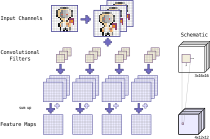
\includegraphics[width=0.6\textwidth]{./4_nn/figs/nn_theory_cnn_basics.eps}
  \caption{Basic CNN layer with a $16 \times 16$ input image, decomposed in 3 channels (CYM) and 4 output feature maps. Kernel size is $5 \times 5$ and the stride is $1$.}
  \label{fig:nn_theory_cnn_basics}
\end{figure}
\FloatBarrier
\noindent


% --
% loss functions

\subsection{Loss Functions and Softmax}
Loss functions or also called cost functions are used to calculate the difference between the predicted labels $\hat{y}$ compared to the actual or ground truth labels $y$.
The predicted labels are usually presented by the output nodes in the last layer of a neural network.
Therefore $\hat{y} = [\hat{y_1}, \, \hat{y_2}, \dots, \hat{y_c}]^T$ has the dimension of the number of labels or classes $c$.
Often it is preferred that $\hat{y} \in R^c$ provides a probability distribution such that:
\begin{equation}
  \sum_{i=0}^c \hat{y}_i = 1
\end{equation}
which can be achieved with the softmax function:
\begin{equation}\label{eq:nn_theory_softmax}
  \hat{y}_i = \frac{\exp{x_i}}{\sum_{j=0}^{c}\exp{x_j}}
\end{equation}
where $c$ is the amount of nodes in this layer, if it is the last layer as usual for the softmax, $c$ is the amount of classes and $\hat{y}_i$ the probability value of the corresponding class $i$.


% --
% dropout

\subsection{Dropout}
Dropout is a method to improve generalization and training of neural network.
The idea is to set the output of randomly selected nodes within a layer and for one training step to zero, so that only the other nodes are updated.
This can be simply done by multiplying all outputs of a current layer with a vector containing a number of zeros and ones places at random positions within the vector.
The amount of zeros compared to ones can be determined by a probability value, for instance $p=0.2$ means that there are 20\% zeros and 80\% ones within the vector.


% --
% training

\subsection{Training of a Neural Network}
The training process of a neural network is usually done with backpropagation of gradients from a loss function at the output nodes.
The backpropagation algorithm is not described here, because there exists many books and papers such as ... with good formulations, further it does not add any value to this thesis as the algorithm is run in the background of all neural network frameworks.
The interesting elements are therefore only the neural network architecture and the loss functions.
